% A little paper on Trapezoidal Shadow Map implementation.
% (c) 2011 Eugene K. Ressler
\documentclass[12pt,letterpaper]{article}
\usepackage{fullpage}
\usepackage{amsmath}
\usepackage{pgf}
\usepackage{tikz}
\usetikzlibrary{arrows,calc}
\usepackage{verbatim}
\usepackage{framed}
\usepackage{biblatex}
\usepackage[small]{caption}
\usepackage{graphicx}
\bibliography{tsm.bib}

\def\pt#1{#1}
\def\vec#1{\mathbf{#1}}
\def\dotprod{\cdot}
\def\zmin{z_{\mathrm{min}}}
\def\zmax{z_{\mathrm{max}}}
\def\coord#1#2{\hbox{$#1$-#2}}

\def\figguts#1#2{\input{fig#1}\caption{#2}\label{fig:#1}}
\def\fig#1#2{
\begin{figure}
\centering
\figguts{#1}{#2}
\end{figure}}

\def\dblfig#1#2#3#4{
\begin{figure}
\begin{minipage}[b]{.5\linewidth}
\centering
\figguts{#1}{#2}
\end{minipage}%
\begin{minipage}[b]{.5\linewidth}
\centering
\figguts{#3}{#4}
\end{minipage}
\end{figure}}

\DeclareMathOperator*{\argmin}{arg\,min}
\DeclareMathOperator*{\argmax}{arg\,max}

\begin{document}
\title{Notes On Implementation Of\\
Trapezoidal Shadow Maps}
\author{Eugene K.\ Ressler}
\date{\today}
\maketitle
\begin{abstract}
The Trapezoidal Shadow Map algorithm by Tobias Martin and Tiow-Seng
Tan is elegant. It deserves equally elegant implementation
details. Here are a few ideas in this regard.
\end{abstract}
\section{Introduction}
We are concerned here with implementation details of trapeziodal
shadow maps as described in~\cite{tobias:2004}, hereinafter called
``the paper.''  The authors, Tobias Martin and Tiow-Seng Tan, have
published some useful ideas of their own~\cite{tobias:2008} including
partial source code~\cite{tobias:code:2004}.  In implementing the
algorithm ourselves, we employed some simplifications. These are
mainly of esthetic interest, which are nonetheless important.  The TSM
algorithm is beautiful and deserves the most beautiful implementation
possible.

\section{Computing the Trapezoid}
The authors' code makes free use of line intersection and inverse
trigonometric function calculations.  We avoid these heavyweight
operations through judicious use of vector products. Our most
expensive arithmetic consists of square roots, and no more than seven
of these to find each trapezoid.

We assume that the view frustum is already transformed to the
post-perspective space of the light (PPSL) as discussed in the paper.
A clear understanding of PPSL will help the reader envision the TSM
algorithm without confusion. PPSL is a two-dimensional space where the
scene could hypothetically be projected to depict what a virtual
observer at the light source would see when looking in the light's
direction. If the light is a point source, perspective division has
already been applied. Otherwise it is a parallel source like the sun,
and the projection is orthogonal. In this case, PPSL is a slight
misnomer because no perspective is involved. The projection boundaries
of the PPSL coordinate system are unimportant because they will be
subsumed in the trapezoidal projection we are about to compute.  This
is why we say ``hypothetical'' above.  PPSL is just a stepping stone
to obtain the final trapezoidal projection. Only the view frustum
world coordinates are transformed to PPSL, not the scene itself.

Figure~\ref{fig:frusta} shows PPSL in our application, which has a
parallel light source.  The clipping boundaries of the projection have
been picked for convenient viewing. Frusta for the viewing and focus
regions are shown in shades of blue.  They are wrapped in the
trapezoid, depicted in green.  Figure~\ref{fig:projection} shows the
same scene after the trapezoidal projection is applied. Objects toward
the viewer are enlarged.%
\begin{figure}
\begin{minipage}[b]{.5\linewidth}
\centering
\includegraphics[width=3in]{frusta.png}
\caption{Frusta and trapezoid in PPSL.}
\label{fig:frusta}
\end{minipage}%
\begin{minipage}[b]{.5\linewidth}
\centering
\includegraphics[width=3in]{projection.png}
\caption{Scene after trapezoidal projection.}
\label{fig:projection}
\end{minipage}
\end{figure}

Though we assume the PPSL convex hull of the view frustum has been
calculated, this is not strictly necessary. Our method ought
to work as well if the eight points of the frustum are processed in
place of four to six convex hull points. The only convex hull that is
strictly necessary is of the focus region so that its area can be
computed when iterating to find the best value of $\eta$ as described
in the paper.

Figure~\ref{fig:T} depicts the view frustum in
gray, already flattened into PPSL coordinates. Points $\pt{N}$ and
$\pt{F}$ are, respectively, the flattened 
centroids of the near and far planes. Then 
the \emph{unit line-of-sight vector} is
\begin{equation}
\vec{a} = \frac{\pt{F} - \pt{N}}{|\pt{F} - \pt{N}|}\;\cdot
\end{equation}
This is a very useful quantity, requiring one square root.

Let points $\pt{P}_i$, $i=1\dotso n$ be the vertices of the convex
hull of the frustum in PPSL. We now compute the dot products
\begin{equation}
t_i = (\pt{P}_i - \pt{N}) \dotprod \vec{a},\quad i=1\dotso n \;.
\end{equation}%
\dblfig{T}{Axis through flattened frustum.}{U}{Hull vertices projected.}
Since these values are signed distances in PPSL measured along vector
$\vec{a}$ from point $\pt{N}$, we can say
\begin{equation}
t_T = \min_i{t_i}\quad\text{and}\quad t_B = \max_i{t_i}
\end{equation}
are, respectively, the distances from $\pt{N}$ to the intersections of
the trapezoid top and base lines with the line-of-sight.
Figure~\ref{fig:U} shows these two intersections projections of all
other convex hull points onto the axis, and the resulting top and
bottom lines. In all but degenerate cases, we will have $t_T<0$ and
$t_B>0$. Two useful facts now arise:
\begin{itemize}
\item
It is never necessary to compute the above intersections. (The authors do.)
\item
Values $t_T$ and $t_B$ are easily computed with one pass over the
convex hull. (The authors use two.)
\end{itemize}

Again because $t_B$ and $t_T$ are distances, $\lambda$ in the paper is
merely
\begin{equation}
\lambda = t_B - t_T \;.
\end{equation}

The next step is to find $\delta'$, the focus distance measured in
PPSL.  The author's code uses a different scheme for computing this
than the one implied by the diagram in the paper, which is merely to
use the distance from the top line to the center of the far plane of
the focus area's truncated frustum,
\begin{equation}
\delta' = t_F - t_T \;.
\end{equation}
The authors used the convex hull of the truncated frustum and the
distance to its farthest point from the top line. The simpler
approach worked well for us.

We turn now to computing the left and right edges.  Use $\lambda$
and $\delta'$ to determine $\eta$ with the simple 80\% formula in the
paper. Point $\pt{Q}$ is then given by
\begin{equation}
\pt{Q} = \pt{N} + (t_T - \eta) \vec{a} \;.
\end{equation}%
\dblfig{V}{Left and right edge directions.}{W}{Complete trapezoid.}

The edge directions are obtained by considering the
rays connecting $\pt{Q}$ to hull vertices as shown in
Figure~\ref{fig:V}.  Their directions are $\pt{P}_i - \pt{Q}$. We
want the leftmost (farthest counter-clockwise) and rightmost (farthest
clockwise) with respect to $\vec{a}$. For this, note that if $\vec{u}$
and $\vec{v}$ are arbitrary unit vectors with included angle $\theta$,
then
\begin{equation}
\sin\theta = x_u y_v - x_v y_u = \vec{u}^\perp \dotprod \vec{v} \;,
\end{equation}
where $\vec{u}^\perp = [-y_u,x_u]$ is $\vec{u}$ rotated by $\pi/2$
radians---the left-perpendicular of $\vec{u}$.  Hence, we compute
\begin{align}
\vec{u}_i &= \frac{\pt{P}_i - \pt{Q}}{|\pt{P}_i - \pt{Q}|} \quad \text{and}
   \label{eqn:unitLR} \\
s_i &= \vec{a}^\perp \dotprod \vec{u}_i \; .
\end{align}
The values $s_i$ are enough to find the desired leftmost and rightmost
rays. The indices are simply
\begin{equation}
L = \argmax_i s_i \quad\text{and}\quad R = \argmin_i s_i \;.  
\end{equation}
No inverse trig functions are needed, only one square root per convex
hull vertex---no more than six.

Let $\vec{u}_L$ and $\vec{u}_R$ be the corresponding leftmost and
rightmost unit vectors, computed previously as $\vec{u}_i$ in
Equation~\ref{eqn:unitLR}.  These are enough to find the four corners
of the trapezoid. In Figure~\ref{fig:solving}, $t$ may be either $t_T
= \eta$, the distance from $\pt{Q}$ to the top line of the trapezoid
or $t_B = \eta + \lambda$, the distance to the base. Vector $\vec{u}$
is either $\vec{u}_L$ or $\vec{u}_R$. Scalar $x$ is the only unknown.
Due to the right angle, we have
\begin{align}
(x\vec{u} - t\vec{a}) \dotprod (t\vec{a}) &= 0 \\
xt(\vec{u} \dotprod \vec{a}) &= t^2 (\vec{a}\dotprod\vec{a}) \\
x &= t / (\vec{u} \dotprod \vec{a}) \;.
\end{align}
This implies that the trapezoid corners $\pt{P}_{TL}$, $\pt{P}_{TR}$,
$\pt{P}_{BR}$, and $\pt{P}_{BL}$ are given by
\begin{equation}
\pt{P}_{ij} = \pt{Q} + \frac{t_i}{\vec{u}_j \dotprod \vec{a}} \vec{u}_j,
\end{equation}
where $i\in\{T,B\}$ and $j\in\{L,R\}$, replacing the author's four
line intersection computations. The result is shown in
Figure~\ref{fig:W}.

The authors use the trapezoidal transformation as the $x$ and $y$
components of the OpenGL projection matrix, setting the $z$ row to
unity.  It is important to remember that front and back clipping will
remove all scene elements outside $[-1..1]$ when writing the depth
buffer.  Either the scene must be appropriately translated and scaled
in $z$ by the model-view matrix, a tricky undertaking if the scene is
lit, or the \coord{z}{row} of the trapezoidal projection must be
modified to do the job.  If this scene lies within extent $[\zmin
  ..\zmax]$ measured from the light (the pseudo eye point used to
transform to PPSL), then the $z$ row should be
\begin{equation}
\left[
\begin{matrix}
0 & 0 & \frac{2}{\zmin - \zmax} & \frac{\zmin + \zmax}{\zmin - \zmax}
\end{matrix}
\right] \;.
\end{equation}%
\begin{figure}
\centering
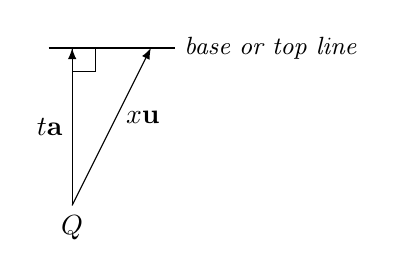
\begin{tikzpicture}[>=latex]
\coordinate [label=below:$Q$] (Q) at (0,0);
\coordinate (A) at (0,2);
\coordinate (B) at (1,2);
\coordinate (Ap) at (-.3,2);
\coordinate [label=right:\emph{\small base or top line}](Bp) at (1.3,2);
\coordinate [label=left:$t\vec{a}$] (QAm) at ($(Q) ! .5 ! (A)$);
\coordinate [label=right:$x\vec{u}$](QBm) at ($(Q) ! .56 ! (B)$);
\draw (A) rectangle (.3,1.7);
\draw [->] (Q) -- (A);
\draw [->] (Q) -- (B);
\draw (Ap) -- (Bp);
\end{tikzpicture}
\caption{Solving for trapezoid corners.}
\label{fig:solving}
\end{figure}%

A final detail is that the computed trapezoid (and rectangle as
discussed below) must be given in a consistent
direction---counterclockwise for default OpenGL processing. A reverse
order will ultimately cause surface normals to also be reversed, which
affects e.g.\ culling. We set out to cull front faces for shadow
map rendering. An early bug was immediately evident as Moir\'e
patterns because back faces were culled instead.

\section{Degenerate Trapezoids}
When the line of sight nearly aligns with the light direction---the
so-called \emph{dueling frustum} case---the focus area is entirely
contained in the far plane, and $\eta$ may become arbitrarily large,
leading to a near-rectangle.  This numerically unstable case can be
repaired by computing a true retangular bounding box whenever $\eta >
k \lambda$ for some $k \gg 1$. The exact value of~$k$ is not critical;
$100$ to $1,000$ work well.  For continuity, alignment with the line
of sight should be maintained.

The top and base lines computed earlier are valid for the bounding box
as well.  We need only the left and right edges.  This time we project
the convex hull vertices onto the left-perpendicular of the unit line
of sight vector.  This provides the signed distance of each vertex
from the line of sight,
\begin{equation}
d_i =\vec{a}^\perp \dotprod  (\pt{P}_i - \pt{N})
\end{equation}
By now our path should be clear. The leftmost and rightmost are given by
\begin{equation}
d_L = \min_i d_i \quad\text{and}\quad d_R = \max_i d_i
\end{equation}
In this case it is convenient to compute the points where the top and
base lines intersect the line of sight,
\begin{equation}
\pt{T} = \pt{N} + t_T\vec{a} \quad\text{and}\quad 
\pt{B} = \pt{N} + t_B\vec{a} \;.
\end{equation}
Then the bounding box corners are just
\begin{equation}
\pt{P}_{ij} = i + d_j\vec{a}^\perp ,
\end{equation}
where again $i\in\{T,B\}$ and $j\in\{L,R\}$.

\section{Trapezoidal Projection Matrix}
We tried an alternative approach just for fun.  The resulting code is
slightly more concise than the authors'.  Figure~\ref{fig:A} dipicts
an arbitrary trapezoid in PPSL. We wish to derive the transformation
that will take it to \coord{x}{$y$} clipping coordinates, which for
OpenGL consist of the square with diagonal $(-1,-1)$ to $(1,1)$.  Note
that in terms of the paper and the previous discussion, edge $P_0P_1$
is the top line, even though here it appears on the bottom. Similarly
$P_2P_3$ is the bottom line.%
\dblfig{A}{Trapezoid in PPSL.}{B}{Translate to origin.}

We begin by translating $P_0$ to the origin as shown in
Figure~\ref{fig:B}.  The required homogeneous transformation matrix
is
\begin{equation}
B = 
\begin{bmatrix}
1 & 0 & -x_{P0} \\
0 & 1 & -y_{P0} \\
0 & 0 & 1
\end{bmatrix} .
\end{equation}

The next step, shown in Figure~\ref{fig:C}, is to rotate the top line
to the \coord{x}{axis}.  
\dblfig{C}{Rotate top edge to \coord{x}{axis}.}
       {D}{Shear to square one corner.}%
For this we note that in finding the trapezoid, we
have already computed the unit line-of-sight vector $\vec{a}$, which
provides the needed cosines for the rotation,
\begin{equation}
C = 
\begin{bmatrix}
y_a & -x_a & 0 \\
x_a &  y_a & 0 \\
0   &  0   & 1
\end{bmatrix} .
\end{equation}
Since we seek an optimized code, pre-multiply by hand to avoid
run-time operations:
\begin{equation}
C B = 
\begin{bmatrix}
y_a & -x_a & x_ay_{P0} - y_ax_{P0} \\
x_a &  y_a & -(x_ax_{P0} + y_ay_{P0}) \\
0   &  0   & 1 
\end{bmatrix} .
\end{equation}
Our approach will be to define variables $m_{ij}$ to contain the
nontrivial portion of the transformation matrix, updating elements
with minimal arithmetic as we proceed with successive
concatenations. Thus, the initial code is
\begin{align}
m_{00}& := y_a & m_{01}& :=-x_a & m_{02}& := x_ay_{P0} - y_ax_{P0} 
\label{code:init}\\
m_{10}& := x_a & m_{11}& := y_a & m_{12}& := -(x_ax_{P0} + y_ay_{P0}) \;. \nonumber
\end{align}

The next step is to shear in $x$ to move point $C_3$ laterally to the
\coord{x}{axis} as shown in Figure~\ref{fig:D}.  To find $C_3$, we use
the transform $CB$ already computed by~(\ref{code:init}) above,
\begin{align}
x_{C3}& := m_{00}x_{P3} + m_{01}y_{P3} + m_{02} \\
y_{C3}& := m_{10}x_{P3} + m_{11}y_{P3} + m_{12} \;. \nonumber
\end{align}
It will be necessary to shear by $-x_{C3}$ in $x$ at $y=y_{C3}$.  The
desired matrix is
\begin{equation}
D = 
\begin{bmatrix}
1 & s & 0 \\
0 & 1 & 0 \\
0 & 0 & 1
\end{bmatrix},\ \text{where}\ s=\frac{-x_{C3}}{y_{C3}} \;.
\end{equation}
We now desire the matrix $DCB$, i.e.\ the first three operations
concatenated. Since we already have $CB$, we would like to know the
necessary update. For this we have
\begin{equation}
D(CB) = 
\begin{bmatrix}
1 & s & 0 \\
0 & 1 & 0 \\
0 & 0 & 1
\end{bmatrix}
\begin{bmatrix}
m_{00} & m_{01} & m_{02} \\
m_{10} & m_{11} & m_{12} \\
0     & 0     & 1
\end{bmatrix}
=
\begin{bmatrix}
m_{00} + s\,m_{10} & m_{01} + s\,m_{11} & m_{02} + s\,m_{12} \\
m_{10} & m_{11} & m_{12} \\
0     & 0     & 1
\end{bmatrix},
\label{eqn:shear}
\end{equation}
which shows that the update is to increment the first row by the
second multiplied by $s$.  In code,
\begin{align}
m_{00}& := m_{00} + s\,m_{10} &
m_{01}& := m_{01} + s\,m_{11} &
m_{02}& := m_{02} + s\,m_{12} \;.
\label{code:shear}
\end{align}
We will repeat this general technique for successive transforms to
follow: Inspect the product $Am=m'$ for each new transform $A$ to
determine minimal arithmetic that computes $m'$ ``in place'' by
carefully modifying the variables $m_{ij}$.

As shown in Figure~\ref{fig:E},%
\dblfig{E}{Translate intersection to origin.}{F}{Scale corner to $(1,1)$.}
we next move the convergence point of the two non-parallel sides in
the positive \coord{y}{direction} to the origin. Point $D_2$ and the
\coord{x}{coordinate} of $D_1$ provide the displacement. The previous
shear operation did not affect \coord{y}{coordinates}.  Therefore
$y_{D2}=y_{C3}$.  The current transformation $DCB$ in
Equation~\ref{eqn:shear} provides the remaining unknowns,
\begin{align}
x_{D1}& := m_{00}x_{P1} + m_{01}y_{P1} + m_{02} \label{eqn:dtwo} \\
x_{D2}& := m_{00}x_{P2} + m_{01}y_{P2} + m_{02} \;. \nonumber
\end{align}

The necessary translation matrix is
\begin{equation}
E = 
\begin{bmatrix}
1 & 0 & 0 \\
0 & 1 & d \\
0 & 0 & 1
\end{bmatrix},\ \text{where}\ 
d = \frac{x_{D1} y_{D2}}{x_{D2} - x_{D1}} \;.
\label{eqn:ydisp}
\end{equation}
Analysis similar to that in Equation~\ref{eqn:shear} provides the
simple update
\begin{equation}
m_{12} := m_{12} + d \;.
\end{equation}
The next operation must scale $E_2$ to (1,1) in preparation for the
perspective-like transformation that will produce a
rectangle. Happily, we can see $x_{E2}=x_{D2}$ and
$y_{E2}=y_{D2}+d$. Therefore the desired matrix is the non-uniform
scaling
\begin{equation}
F =
\begin{bmatrix}
s_x &   0 & 0 \\
0   & s_y & 0 \\
0   &   0 & 1 
\end{bmatrix},\quad\text{where}\quad
s_x = 1/x_{E2}\ \text{and}\ s_y = 1/y_{E2} \;,
\end{equation}
and the needed update to obtain the next step $FEDCB$ is six
multiplications.
\begin{align}
m_{00}& := s_x\,m_{00} & 
m_{01}& := s_x\,m_{01} & 
m_{02}& := s_x\,m_{02} \label{eqn:scalexy} \\
m_{10}& := s_y\,m_{10} & 
m_{11}& := s_y\,m_{11} & 
m_{12}& := s_y\,m_{12}
\nonumber
\end{align}

The handiest form for the perspective transformation seems to be
\begin{equation}
G =
\begin{bmatrix}
  1 & 0 &  0 \\
  0 & 1 & -1 \\
  0 & 1 &  0
\end{bmatrix},
\end{equation}
with the result shown in Figure~\ref{fig:G}.
This%
\dblfig{G}{Perspective along \coord{y}{axis}.}
       {H}{Scale and translate to clip box.}
both rectifies the quad and avoids topological mirroring.
Pre-multiplying this matrix to form $G(FEDCB)$ copies the second row
of the previous matrix to the third, which has until now remained as
$[0,0,1]$. Then it subtracts one from the last element of the second
row. The update is
\begin{align}
m_{20}& := m_{10} & m_{21}& := m_{11} & m_{22}& := m_{12} 
\label{eqn:persp}\\
     &          &       &          & m_{12}& := m_{12} - 1 
\;. \nonumber
\end{align}

In the final matrix, we combine scaling followed by translation to
gain the desired square in one step.  The reader will easily verify
that the needed matrix is
\begin{equation}
H = 
\begin{bmatrix}
2 & 0 & -1 \\
0 & u &  1 \\
0 & 0 &  1
\end{bmatrix},\ \text{where}\ u = \frac{-2}{y_{G0}} \;.
\label{eqn:ygz}
\end{equation}
The corresponding update is a bit more complicated than previous ones
because the last row of the accumulated matrix is no longer a unit-$z$
transformation,
\begin{align}
m_{00}& := 2\,m_{00} - m_{20} &
m_{01}& := 2\,m_{01} - m_{21} &
m_{02}& := 2\,m_{02} - m_{22} \label{eqn:final} \\
m_{10}& := u\,m_{10} + m_{20} &
m_{11}& := u\,m_{11} + m_{21} &
m_{12}& := u\,m_{12} + m_{22} \;. \nonumber
\end{align}

Additional economy is possible by noting that Updates~\ref{eqn:final} and
\ref{eqn:scalexy} both scale entire rows. Composing $H$, $G$, and $F$ in
a single transform on $m=EDCB$ produces
\begin{equation}
HGFm =
\begin{bmatrix}
2     s_x m_{00} - s_y m_{10} &
2     s_x m_{01} - s_y m_{11} &
2     s_x m_{02} - s_y m_{12} \\
(u+1) s_y m_{10} &
(u+1) s_y m_{11} &
(u+1) s_y m_{12} - u \\
      s_y m_{10} &
      s_y m_{11} &
      s_y m_{12}
\end{bmatrix} .
\end{equation}
Here the third row contains terms that are repeated in the other
two. Consequently, careful ordering provides a bit more efficiency
than the sequence of Updates~\ref{eqn:scalexy}, \ref{eqn:persp},
\ref{eqn:final} that this single one replaces.
\begin{align}
m_{20}& := m_{10} s_y &
m_{21}& := m_{11} s_y &
m_{22}& := m_{12} s_y \\
m_{10}& := (u+1) m_{20} &
m_{11}& := (u+1) m_{21} &
m_{12}& := (u+1) m_{22} - u \nonumber \\
m_{00}& := (2 s_x) m_{00} - m_{20} &
m_{01}& := (2 s_x) m_{01} - m_{21} &
m_{02}& := (2 s_x) m_{02} - m_{22} \nonumber
\end{align}
The factors in parentheses should be optimized by the compiler to
eliminate redundant computations.

The remaining detail is to compute $y_{G0}$, which is needed in
Equation~\ref{eqn:ygz}. Observe $y_{E0}=d$, where $d$ was computed in
Equation~\ref{eqn:ydisp}.  Thus we need only to find the product,
\begin{equation}
FG\begin{bmatrix} 0 \\ d \\ 1 \end{bmatrix}
= \begin{bmatrix} 0 \\ s_y\,d - 1 \\ s_y\,d \end{bmatrix}.
\end{equation}
Perspective division to obtain the true coordinate produces
\begin{equation}
u = \frac{-2}{y_{G0}} 
= \frac{2 s_y d}{1 - s_y d} \;.
\end{equation}

\section{Degenerate Trapezoids, A Reprise}
Again a numerically unstable case occurs when the trapezoid is nearly
rectangular. Referring to Equation~\ref{eqn:ydisp}, for such a
trapezoid $d \gg 1$, causing translation $E$ to move the quad
arbitrarly far from the origin.

The solution is to replace $E$ with a new transform that maps the
rectangle with diagonal from the origin to $D_2$ to our target
square. This is certain to cover the frustum even when the bounding
quad is slightly tapered.

The value of $D_2$ is already on hand from Equation~\ref{eqn:dtwo}.
The desired matrix is similar to $H$ in Equation~\ref{eqn:ygz},
\begin{equation}
E' = 
\begin{bmatrix}
s'_x & 0 & -1 \\
0 & s'_y & -1 \\
0 & 0    &  1
\end{bmatrix},\ \text{where}\ 
s'_x = \frac{2}{x_{D2}}\ \text{and}\
s'_y = \frac{2}{y_{D2}} \;.
\end{equation}
The update is simple, and we must also fill in the third matrix row,
\begin{align}
m_{00}& := s'_x\,m_{00} & 
m_{01}& := s'_x\,m_{01} & 
m_{02}& := s'_x\,m_{02} - 1 \\
m_{10}& := s'_y\,m_{10} & 
m_{12}& := s'_y\,m_{11} & 
m_{12}& := s'_y\,m_{12} - 1 \nonumber \\
m_{20}& := 0 &
m_{21}& := 0 &
m_{22}& := 1 \;. \nonumber
\end{align}

\section{Correcting $z$}
The authors use shader programs to undo distortion in
\coord{z}{coordinates} introduced by the trapezoidal
transformation. Portability is a difficult and important problem for
our application, so we sought to avoid shaders.

We found that by culling front faces during shadow map construction
and carefully centering the scene at the origin, we obtained
acceptable results with no \coord{z}{correction}.  Minor acne on some
shadowed faces was the only flaw.  Our light source is parallel.  This
may be an advantage.

An additional problem caused by \coord{z}{coordinate} distortion
beyond shadow map offset is its effect on front and back
clipping. When we originally positioned the eye point at a virtual
light source point far ``outside'' the scene while rendering the
shadow map, \coord{z}{distortion} was so great that front and back
clipping removed arbitrary chunks of scene from the shadow map.  Since
corresonding depth information was missing in the rendering pass,
portions of shadows to randomly disappeared in the scene.  This
changed with the trapezoid shape as the viewer's eye moved.  It took a
day to figure out what was going on! When we set front and back planes
far apart to prevent clipping, it was very far indeed. This caused
poor shadows due to inadequate depth resolution.  The problem was
solved by changing the shadow mapping eye point to the center of the
scene---possible due to our parallel light source.  With this,
distortion decreased enough for the algorithm give good results with
no $z$-component correction as mentioned above.

\section{Results and Code}
In Figure~\ref{fig:A} the green-shaded tiles are closest to the
frustum eye point.  Yellow and red are successively farther away.  In
Figure~\ref{fig:H} the green tiles cover far larger areas, while the
red ones have shrunk. This is precisely the intent of the TSM
algorithm.

Our implementation is for the West Point Bridge Designer, 2nd Edition.
A scene is shown in Figure~\ref{fig:bdscene}.
\begin{figure}
\centering
\includegraphics[width=6in]{scene.png}
\caption{A shadowed scene from the West Point Bridge Designer.}
\label{fig:bdscene}
\end{figure}

In Figure~\ref{fig:code}, we implement the logic above in C code, but
in a form where the fragment that computes $m$ will transpose easily
to many other languages. We have used it in Java, for example.
\begin{figure}
\footnotesize
\begin{quote}
\begin{verbatim}
#include <stdio.h>
#include <math.h>
void trapezoid_to_clip(double xp0, double yp0, double xp1, double yp1,
                       double xp2, double yp2, double xp3, double yp3) {
  double m00, m01, m02, m10, m11, m12, m20, m21, m22;
  double xa, ya, xc3, yc3, s, xd1, xd2, d, sx, sy, u;

  // Not needed in TSM algorithm: unit LOS vector already computed.
  double dx = xp1 - xp0; double dy = yp1 - yp0;
  double len = sqrt(dx * dx + dy * dy);
  xa = -dy / len; ya = dx / len;

  // ----- Begin fragment to find m. -------------------------------------------
  m00 = ya; m01 = -xa; m02 =   xa * yp0 - ya * xp0;     //                  (23)
  m10 = xa; m11 =  ya; m12 = -(xa * xp0 + ya * yp0);
  xc3 = m00 * xp3 + m01 * yp3 + m02;                    //                  (24)
  yc3 = m10 * xp3 + m11 * yp3 + m12;
  s = -xc3 / yc3;                                       //                  (25)
  m00 += s * m10; m01 += s * m11; m02 += s * m12;       //                  (27)
  xd1 = m00 * xp1 + m01 * yp1 + m02;                    //                  (28)
  xd2 = m00 * xp2 + m01 * yp2 + m02;
  d = yc3 / (xd2 - xd1);                                // yd2 = yc3, start (29)
  if (0 <= d && d < 1e4) {  // Trapezoid case.
    d *= xd1; m12 += d;                                 //           finish (29)
    sx = 2 / xd2; sy = 1 / (yc3 + d);                   //   ye2=yd2=yc3 in (31)
    u = (2 * (sy * d)) / (1 - (sy * d));                //                  (34)
    m20 = m10 * sy;       m21 = m11 * sy;       m22 = m12 * sy; //          (38)
    m10 = (u + 1) * m20;  m11 = (u + 1) * m21;  m12 = (u + 1) * m22 - u;
    m00 = sx * m00 - m20; m01 = sx * m01 - m21; m02 = sx * m02 - m22;
  } else {                  // Near-rectangle case.
    sx = 2 / xd2; sy = 2 / yc3;                         //     yd2 = yc3 in (41)
    m00 *= sx; m01 *= sx; m02 = m02 * sx - 1;
    m10 *= sy; m11 *= sy; m12 = m12 * sy - 1;
    m20 = 0;   m21 = 0;   m22 = 1;
  } // --- Done with fragment to find m. ---------------------------------------
  // Do a trivial test.
#define TRANSFORM_AND_PRINT(P) do {\
    double w = (m20 * x##P + m21 * y##P + m22);\
    double x = (m00 * x##P + m01 * y##P + m02) / w;\
    double y = (m10 * x##P + m11 * y##P + m12) / w;\
    printf(#P " -> (%6.3f, %6.3f)\n", x, y); } while (0)
  TRANSFORM_AND_PRINT(p0); TRANSFORM_AND_PRINT(p1);
  TRANSFORM_AND_PRINT(p2); TRANSFORM_AND_PRINT(p3);
}
int main(void) {
  trapezoid_to_clip(2, 1,   4, 0,   7, 1,  0, 4.5);
  trapezoid_to_clip(1, 1,   3, 2,   2, 4,  0, 3);
  return 0;
}
\end{verbatim}
\end{quote}
\caption{C code with easily portable fragment to compute $m$.}
\label{fig:code}
\end{figure}
\printbibliography
\end{document}
